\documentclass[12pt]{report}
\usepackage[utf8]{inputenc}
\usepackage[russian]{babel}
%\usepackage[14pt]{extsizes}
\usepackage{listings}
\usepackage{graphicx}
\usepackage{amsmath,amsfonts,amssymb,amsthm,mathtools} 
\usepackage{pgfplots}
\usepackage{filecontents}
\usepackage{indentfirst}
\usepackage{eucal}
\usepackage{amsmath}
\usepackage{enumitem}
\frenchspacing

\usepackage{indentfirst} % Красная строка


%\usetikzlibrary{datavisualization}
%\usetikzlibrary{datavisualization.formats.functions}

\usepackage{amsmath}




% Для листинга кода:
\lstset{ %
language=haskell,                 % выбор языка для подсветки (здесь это С)
basicstyle=\small\sffamily, % размер и начертание шрифта для подсветки кода
numbers=left,               % где поставить нумерацию строк (слева\справа)
numberstyle=\tiny,           % размер шрифта для номеров строк
stepnumber=1,                   % размер шага между двумя номерами строк
numbersep=5pt,                % как далеко отстоят номера строк от подсвечиваемого кода
showspaces=false,            % показывать или нет пробелы специальными отступами
showstringspaces=false,      % показывать или нет пробелы в строках
showtabs=false,             % показывать или нет табуляцию в строках
frame=single,              % рисовать рамку вокруг кода
tabsize=2,                 % размер табуляции по умолчанию равен 2 пробелам
captionpos=t,              % позиция заголовка вверху [t] или внизу [b] 
breaklines=true,           % автоматически переносить строки (да\нет)
breakatwhitespace=false, % переносить строки только если есть пробел
escapeinside={\#*}{*)}   % если нужно добавить комментарии в коде
}

\usepackage[left=2cm,right=2cm, top=2cm,bottom=2cm,bindingoffset=0cm]{geometry}
% Для измененных титулов глав:
\usepackage{titlesec, blindtext, color} % подключаем нужные пакеты
\definecolor{gray75}{gray}{0.75} % определяем цвет
\newcommand{\hsp}{\hspace{20pt}} % длина линии в 20pt
% titleformat определяет стиль
\titleformat{\chapter}[hang]{\Huge\bfseries}{\thechapter\hsp\textcolor{gray75}{|}\hsp}{0pt}{\Huge\bfseries}


% plot
\usepackage{pgfplots}
\usepackage{filecontents}
\usetikzlibrary{datavisualization}
\usetikzlibrary{datavisualization.formats.functions}
\RequirePackage[
  style=gost-numeric,
  language=auto,
  autolang=other,
  sorting=none,
]{biblatex}

\addbibresource{bib.bib}
\begin{document}
%\def\chaptername{} % убирает "Глава"
\thispagestyle{empty}
\begin{titlepage}
	\noindent \begin{minipage}{0.15\textwidth}
	
\includegraphics[width=\linewidth]{b_logo}
	\end{minipage}
	\noindent\begin{minipage}{0.9\textwidth}\centering
		\textbf{Министерство науки и высшего образования Российской Федерации}\\
		\textbf{Федеральное государственное бюджетное образовательное учреждение высшего образования}\\
		\textbf{~~~«Московский государственный технический университет имени Н.Э.~Баумана}\\
		\textbf{(национальный исследовательский университет)»}\\
		\textbf{(МГТУ им. Н.Э.~Баумана)}
	\end{minipage}
	
	\noindent\rule{18cm}{3pt}
	\newline\newline
	\noindent ФАКУЛЬТЕТ $\underline{\text{«Информатика и системы управления»}}$ \newline\newline
	\noindent КАФЕДРА $\underline{\text{«Программное обеспечение ЭВМ и информационные технологии»}}$\newline\newline\newline\newline\newline
	
	
	\begin{center}
		\noindent\begin{minipage}{1.3\textwidth}\centering
			\Large\textbf{  Отчёт по лабораторным работам №2 по дисциплине}\newline
			\textbf{ "Методы машинного обучения"}\newline\newline
		\end{minipage}
	\end{center}
	
	\noindent\textbf{Тема} $\underline{\text{Модель полиномиальной регрессии - Регуляризация.}}$\newline\newline
	\noindent\textbf{Студент} $\underline{\text{Варламова Е. А.}}$\newline\newline
	\noindent\textbf{Группа} $\underline{\text{ИУ7-23М}}$\newline\newline
	\noindent\textbf{Оценка (баллы)} $\underline{\text{~~~~~~~~~~~~~~~~~~~~~~~~~~~}}$\newline\newline
	\noindent\textbf{Преподаватели} $\underline{\text{Солодовников Владимир Игоревич}}$\newline\newline\newline
	
	\begin{center}
		\vfill
		Москва~---~\the\year
		~г.
	\end{center}
\end{titlepage}
\large
\setcounter{page}{2}
\def\contentsname{СОДЕРЖАНИЕ}
\renewcommand{\contentsname}{СОДЕРЖАНИЕ}
\tableofcontents
\renewcommand\labelitemi{---}
\newpage
\chapter{Теоретическая часть}
\section{Полиномиальная регрессия. Регуляризация.}

Полиномиальная регрессия -- это метод восстановления зависимости между независимыми и зависимыми переменными при помощи полиномиальной функции. Он часто используется для приближения нелинейного поведения данных и улучшения качества предсказаний по сравнению с линейной регрессией. Полиномиальная регрессия позволяет уловить сложные взаимосвязи в данных и учитывать нелинейные зависимости.

Регуляризация в статистике и машинном обучении -- метод добавления некоторых дополнительных ограничений к условию с целью предотвратить переобучение. Чаще всего эта информация имеет вид штрафа за сложность модели.

Целью данной лабораторной работы является применение регуляризации к модели полиномиальной регрессии.

Для этого необходимо решить следующие задачи:
\begin{itemize}
    \item формализовать задачу;
    \item описать алгоритм работы ПО, решающего поставленную задачу;
    \item привести особенности реализации ПО, решающего поставленную задачу;
    \item провести исследование зависимости среднеквадратичной ошибки регрессии от степени полинома;
    \item провести исследование зависимости значения функционала эмпирического риска на обучающей и контрольной выборках от степени полинома.
\end{itemize}

\section{Постановка задачи}

Функция:
\begin{equation}
    y(x) = \frac{1}{1 + 25x^2}, x \in [-2,2]
\end{equation}

Обучающая выборка:
\begin{equation}
S_l: x_i = \frac{4(i-1)}{l-1} - 2, i=1,\ldots,l 
\end{equation}

Контрольная выборка:
\begin{equation}
S_k: x_i = \frac{4(i-0.5)}{l-1} - 2, i=1,\ldots,l-1.
\end{equation}

Построить модель полиномиальной регрессии, аппроксимирующей данные обучающей выборки. Исходить из того, что степень полинома (начальный закон генерации обучающей выборки) неизвестен. 
Обучение проводить методом наименьших квадратов.

Для оптимальной модели полиномиальной регрессии, а также для модели полиномов меньшей и большей  степеней (±3) вывести значения коэффициентов полинома (всего 3 полинома). 

К выбранным моделям (полиномам соответствующих степеней) применить метод регуляризации с использованием гребневой регрессии (ридж-регрессии) и Лассо-регрессии. Вывести значения коэффициентов полинома. Повторить для различных значений параметра λ.

Рассчитать функционал эмпирического риска (функционал качества) для всех полученных моделей на обучающей и контрольной выборках (вывести графики).


\section{Функционал эмпирического риска}

Функционал эмпирического риска (empirical risk functional) используется в машинном обучении для измерения качества модели на обучающей выборке. Он представляет собой среднее значение функции потерь (loss function) на обучающих примерах.

Для задачи регрессии, наши данные состоят из пар $(x_i, y_i)$, где $x_i$ - входное значение, а $y_i$ - соответствующее целевое значение. Пусть $h(x)$ - модель, а $\ell(h(x), y)$ - функция потерь. Тогда эмпирический риск $R(h)$ может быть записан следующим образом:

\begin{equation*}
R(h) = \frac{1}{N} \sum_{i=1}^{N} \ell(h(x_i), y_i)
\end{equation*}

Здесь $N$ - количество обучающих примеров, и сумма берется по всем парам $(x_i, y_i)$. Функция потерь $\ell(h(x_i), y_i)$ оценивает разницу между предсказанным значением $h(x_i)$ и истинным значением $y_i$. 

\textbf{В данной работе используется квадратичная функция потерь, а, соотвественно, функционал эмпирического риска равен среднеквадратичной ошибке.} 

\section{Регуляризация}
Регуляризация  в статистике и машинном обучении -- метод добавления некоторых дополнительных ограничений к условию с целью предотвратить переобучение. Чаще всего эта информация имеет вид штрафа за сложность модели.

Если выбрана излишне сложная модель при недостаточном объеме данных, то в итоге может быть получена модель, которая хорошо описывает обучающую выборку, но не обобщается на тестовую. Переобучение в большинстве случаев проявляется в том, что итоговые модели имеют слишком большие значения параметров. Одним из способов борьбы с негативным эффектом излишнего подстраивания под данные -- использование регуляризации, т.е. добавление некоторого штрафа за большие значения коэффициентов у линейной модели. Тем самым запрещаются слишком "резкие" изгибы, и предотвращается переобучение.

Наиболее часто используемые виды регуляризации — $L_1$ и $L_2$, а также их линейная комбинация -- эластичная сеть. 

В представленных ниже формулах для эмпирического риска Q приняты следующие обозначения: $L$ -- функция потерь, $\beta$ -- вектор параметров $g(x,\beta)$ из модели алгоритма, $\lambda$ -- неотрицательный гиперпараметр (коэффициент регуляризации).

Если в качестве функционал качества используется сумма квадратов остатков (Residual Sum of Squares -- RSS), тогда изначально: 

\begin{equation}
    L(y_i, g(x_i, \beta)) = (g(x_i, \beta) - y_i)^2
\end{equation}
\begin{equation}
RSS=Q(\beta,X^l )=\sum_{i=1}^l(L(y_i,g(x_i,\beta)))=\sum_{i=1}^l(g(x_i,\beta)-y_i )^2 
\end{equation}

$L_2$-регуляризация (ridge regularization) или регуляризация Тихонова (Tikhonov regularization):

\begin{equation}
Q(\beta,X^l )=\sum_{i=1}^l L(y_i,g(x_i,\beta)) + \lambda \sum_{j=1}^n \beta_j^2 
\end{equation}

Минимизация регуляризованного cоответствующим образом эмпирического риска приводит к выбору такого вектора параметров $\beta$, которое не слишком сильно отклоняется от нуля. В линейных классификаторах это позволяет избежать проблем мультиколлинеарности и переобучения.

$L_1$-регуляризация (lasso regularization) или регуляризация через манхэттенское расстояние:

\begin{equation}
Q(\beta,X^l )=\sum_{i=1}^l L(y_i,g(x_i,\beta)) + \lambda \sum_{j=1}^n |\beta_j|
\end{equation}

Данный вид регуляризации также позволяет ограничить значения вектора $\beta$. Однако, к тому же он обладает интересным и полезным на практике свойством -- обнуляет значения некоторых параметров, что в случае с линейными моделями приводит к отбору признаков.
\section{Описание алгоритма}
Схема алгоритма, вычисляющего оптимальную степень полинома по обучающей выборке, представлена на рисунке \ref{fig:algo_gen}. 

\begin{figure}[h!]
  \centering
  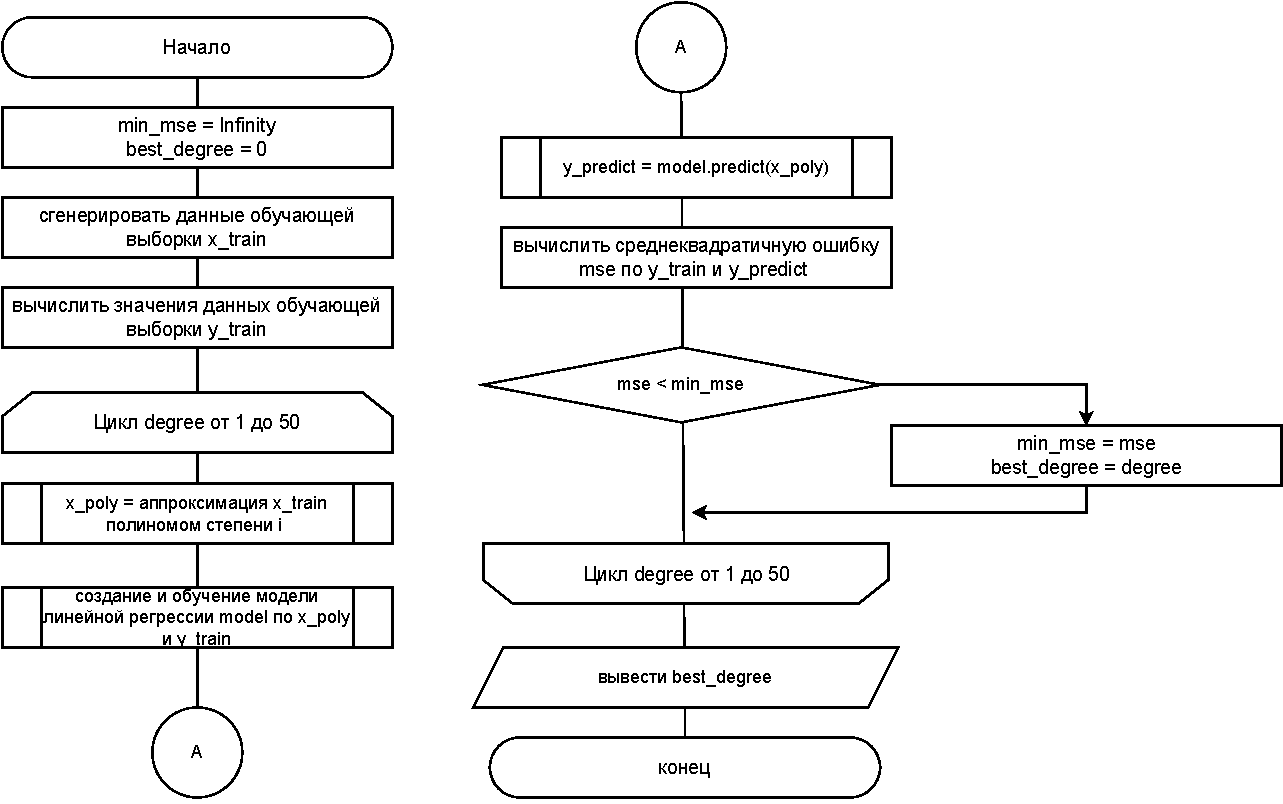
\includegraphics[width = \linewidth]{mml_lab_01.pdf}
  \caption{Схема работы алгоритма}
  \label{fig:algo_gen}
\end{figure}


\chapter{Практическая часть}

\section{Выбор средств разработки}
В качестве языка программирования был использован язык Python, поскольку этот язык кроссплатформенный и для него разработано огромное количество библиотек и модулей, решающих разнообразные задачи. 

В частности, имеются библиотеки, включающие в себя алгоритмы аппроксимации полиномом, линейной регрессии и регуляризации в библиотеке \cite{bib:sklearn}.

Для создания графиков была выбрана библиотека matplotlib \cite{bib:matplotlib}, доступная на языке Python, так как она предоставляет удобный интерфейс для работы с данными и их визуализации.

\section{Исследование ПО}

В листинге \ref{lst:gen} представлен код, выводящий максимальное по модулю значение коэффициентов полинома и значение ошибок на обучающей и контрольной выборок для моделей полиномиальной регрессии без регуляризации и с регуляризацией с помощью Лассо и Ридж методов для степеней полинома 10, 13 и 20 и для разных параметров $\alpha$. Кроме того, для указанных моделей предусмотрен интерфейс вывода графиков фнукционала эмпирического риска в зависимости от степени полинома с возможностью варьировать параметры методов регуляризации.

\begin{lstlisting}[label=lst:gen,caption=код, решающий поставленную задачу]
import numpy as np
import matplotlib.pyplot as plt
from sklearn.preprocessing import PolynomialFeatures
from sklearn.linear_model import LinearRegression
from sklearn.metrics import mean_squared_error
from sklearn.linear_model import Ridge
from sklearn.linear_model import Lasso
from matplotlib.widgets import Slider
import warnings
warnings.filterwarnings("ignore")
def true_function(x):
    return 1 / (1 + 25 * x**2)

l = 21
X_train = np.array([4 * (i - 1) / (l - 1) - 2 for i in range(1, l + 1)]).reshape(-1, 1)
X_control = np.array([4 * (i - 0.5) / (l - 1) - 2 for i in range(1, l)]).reshape(-1, 1)
y_train = true_function(X_train)
y_control = true_function(X_control)
degrees = [10, 13, 16]
def fit_polynomial_regression(X, y, degree, model):
    poly_features = PolynomialFeatures(degree=degree)
    X_poly = poly_features.fit_transform(X)
    model.fit(X_poly, y)
    return poly_features


def calculate_error(model, poly_features, X, y):
    X_poly = poly_features.transform(X)
    y_pred = model.predict(X_poly)
    return mean_squared_error(y, y_pred), y_pred
def get_errs(model, X_train, y_train, X_control, y_control):
    train_errors = []
    control_errors = []
    for degree in degrees:
        poly_features = fit_polynomial_regression(X_train, y_train, degree, model)
        train_error, y_p_t = calculate_error(model, poly_features, X_train, y_train)
        control_error, y_p_c = calculate_error(model, poly_features, X_control, y_control)
        train_errors.append(train_error)
        control_errors.append(control_error)
    return train_errors,control_errors

def update_ridge(val):
    train_errors_ridge, control_errors_ridge = get_errs(Ridge(alpha=val), X_train, y_train, X_control, y_control)
    ridge_plot_train.set_ydata(train_errors_ridge)
    ridge_plot_control.set_ydata(control_errors_ridge)
    fig.canvas.draw_idle()
    
def update_lasso(val):
    train_errors_lasso, control_errors_lasso = get_errs(Lasso(alpha=val), X_train, y_train, X_control, y_control)
    lasso_plot_train.set_ydata(train_errors_lasso)
    lasso_plot_control.set_ydata(control_errors_lasso)
    fig.canvas.draw_idle()

def output_errors():
    models = [LinearRegression(),
              Lasso(alpha=0.1),
              Lasso(alpha=10),
              Lasso(alpha=100),
              Lasso(alpha=1000),
              Ridge(alpha=0.1),
              Ridge(alpha=10),
              Ridge(alpha=100),
              Ridge(alpha=1000)]
    names = ["Линейная",
             "Лассо, alpha = 0.1",
             "Лассо, alpha = 10",
             "Лассо, alpha = 100",
             "Лассо, alpha = 1000",
             "Ридж, alpha = 0.1",
             "Ридж, alpha = 10",
             "Ридж, alpha = 100",
             "Ридж, alpha = 1000"]
    degs = [10, 13, 20]
    i = 0
    for model in models:
        for degree in degs:
            poly_features = fit_polynomial_regression(X_train, y_train, degree, model)
            train_error, y_p_t = calculate_error(model, poly_features, X_train, y_train)
            control_error, y_p_c = calculate_error(model, poly_features, X_control, y_control)
            print("\hline {} & {} & {:.3f} & {:.3f} & {:.3f} & {:.3f} \\\\".format(names[i],
                                                                 degree,
                                                                 np.max(np.abs(y_p_t)),
                                                                 np.max(np.abs(y_p_c)),
                                                                 train_error,
                                                                 control_error))
        i += 1
output_errors()
fig, ax = plt.subplots()

ax_slider_ridge = plt.axes([0.1, 0.01, 0.8, 0.03])
ax_slider_lasso = plt.axes([0.1, 0.9, 0.8, 0.03])

train_errors_lin, control_errors_lin = get_errs(LinearRegression(), X_train, y_train, X_control, y_control)
ax.plot(degrees, train_errors_lin, label='Обучающая выборка, линейная')
ax.plot(degrees, control_errors_lin, label='Контрольная выборка, линейная')

train_errors_lasso, control_errors_lasso = get_errs(Lasso(alpha=0.1), X_train, y_train, X_control, y_control)
lasso_plot_train,  = ax.plot(degrees, train_errors_lasso, label='Обучающая выборка, лассо')
lasso_plot_control,  = ax.plot(degrees, control_errors_lasso, label='Контрольная выборка, лассо')

train_errors_ridge, control_errors_ridge = get_errs(Ridge(alpha=0.1), X_train, y_train, X_control, y_control)
ridge_plot_train,  = ax.plot(degrees, train_errors_ridge, label='Обучающая выборка, ридже')
ridge_plot_control,  = ax.plot(degrees, control_errors_ridge, label='Контрольная выборка, ридже')

slider_ridge = Slider(ax_slider_ridge, 'Ridge', valmin=0, valmax=1000, valinit=0.1)
slider_ridge.on_changed(update_ridge)

slider_lasso = Slider(ax_slider_lasso, 'Lasso', valmin=0, valmax=1000, valinit=0.1)
slider_lasso.on_changed(update_lasso)
ax.legend()

plt.xlabel('Степень полинома')
plt.ylabel('Значение ошибки')
plt.title('Зависимость значения ошибки от степени полинома')
plt.legend()
plt.show()


\end{lstlisting}

На рисунке \ref{fig:points5} показана зависимость значения ошибки от степени полинома для обучающей и контрольной выбоорок для разных моделей.

\begin{figure}[H!]
  \centering
  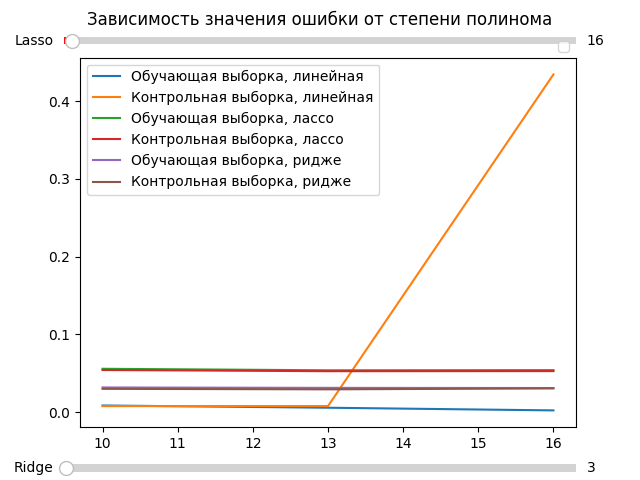
\includegraphics[width = \linewidth]{f1.png}
  \caption{}
  \label{fig:points5}
\end{figure}

В таблице \ref{tbl1} показано, что при применении методов регуляризации максимальный по модулю коэффициент не такой большой, как без регуляризации.

\begin{table}[!h]
	\begin{center}
		\caption{\label{tbl1}Результаты работы ПО} 
		\footnotesize
		\begin{tabular}{|l|l|l|l|l|l|}
			\hline	
   \multicolumn{1}{|c|}{\begin{tabular}[c]{@{}c@{}}Тип \\ модели\end{tabular}} & 
   \multicolumn{1}{c|}{\begin{tabular}[c]{@{}c@{}}Степень \\ полинома \end{tabular}} & 
    \multicolumn{1}{c|}{\begin{tabular}[c]{@{}c@{}}max модуль \\ коэффициента\\ полинома \\ на обучающей \\ выборке\end{tabular}} & 
    \multicolumn{1}{c|}{\begin{tabular}[c]{@{}c@{}}max модуль \\ коэффициента\\ полинома \\ на контрольной \\ выборке\end{tabular}} & 
   \multicolumn{1}{c|}{\begin{tabular}[c]{@{}c@{}}Ошибка на\\  обучающей \\ выборке\end{tabular}} & 
   \multicolumn{1}{c|}{\begin{tabular}[c]{@{}c@{}}Ошибка на\\  контрольной \\ выборке\end{tabular}}  \\
\hline Линейная & 5 & 0.415 & 0.411 & 0.027 & 0.025 \\
\hline Линейная & 10 & 0.692 & 0.665 & 0.008 & 0.008 \\
\hline Линейная & 20 & 1.000 & 360.683 & 0.000 & 13108.005 \\
\hline Лассо, alpha = 0.1 & 5 & 0.199 & 0.199 & 0.048 & 0.047 \\
\hline Лассо, alpha = 0.1 & 10 & 0.211 & 0.211 & 0.047 & 0.045 \\
\hline Лассо, alpha = 0.1 & 20 & 0.217 & 0.217 & 0.046 & 0.044 \\
\hline Лассо, alpha = 10 & 5 & 0.141 & 0.141 & 0.057 & 0.055 \\
\hline Лассо, alpha = 10 & 10 & 0.155 & 0.155 & 0.054 & 0.053 \\
\hline Лассо, alpha = 10 & 20 & 0.177 & 0.177 & 0.052 & 0.051 \\
\hline Лассо, alpha = 100 & 5 & 0.141 & 0.141 & 0.057 & 0.055 \\
\hline Лассо, alpha = 100 & 10 & 0.141 & 0.141 & 0.057 & 0.055 \\
\hline Лассо, alpha = 100 & 20 & 0.160 & 0.160 & 0.054 & 0.053 \\
\hline Лассо, alpha = 1000 & 5 & 0.141 & 0.141 & 0.057 & 0.055 \\
\hline Лассо, alpha = 1000 & 10 & 0.141 & 0.141 & 0.057 & 0.055 \\
\hline Лассо, alpha = 1000 & 20 & 0.158 & 0.158 & 0.055 & 0.054 \\
\hline Ридж, alpha = 0.1 & 5 & 0.408 & 0.404 & 0.027 & 0.025 \\
\hline Ридж, alpha = 0.1 & 10 & 0.494 & 0.486 & 0.018 & 0.016 \\
\hline Ридж, alpha = 0.1 & 20 & 0.511 & 1.432 & 0.016 & 0.226 \\
\hline Ридж, alpha = 10 & 5 & 0.258 & 0.257 & 0.040 & 0.038 \\
\hline Ридж, alpha = 10 & 10 & 0.287 & 0.286 & 0.036 & 0.034 \\
\hline Ридж, alpha = 10 & 20 & 0.296 & 0.296 & 0.036 & 0.034 \\
\hline Ридж, alpha = 100 & 5 & 0.212 & 0.211 & 0.046 & 0.045 \\
\hline Ридж, alpha = 100 & 10 & 0.230 & 0.229 & 0.044 & 0.043 \\
\hline Ридж, alpha = 100 & 20 & 0.249 & 0.407 & 0.042 & 0.058 \\
\hline Ридж, alpha = 1000 & 5 & 0.170 & 0.170 & 0.051 & 0.050 \\
\hline Ридж, alpha = 1000 & 10 & 0.201 & 0.201 & 0.048 & 0.046 \\
\hline Ридж, alpha = 1000 & 20 & 0.220 & 0.220 & 0.046 & 0.046 \\
\hline
	\end{tabular}
	\end{center}
\end{table}

\printbibliography[title={СПИСОК ИСПОЛЬЗОВАННЫХ\\ ИСТОЧНИКОВ}]
\addcontentsline{toc}{chapter}{СПИСОК ИСПОЛЬЗОВАННЫХ ИСТОЧНИКОВ}

\end{document}